\documentclass[a4paper,12pt]{report}
% safe参数解决与\!在内的多个冲突
% \sups命令可能被重定义,xeCJK放在tipa后
\usepackage[safe]{tipa}
\usepackage{algorithm}
\usepackage{amsmath,bm}
\usepackage{algorithmic}
\usepackage{fancybox}
\usepackage{listings}
\usepackage{xcolor}
\usepackage{diagbox}
\usepackage{amssymb}
\usepackage{amsmath}
\usepackage{amsthm}
\usepackage{empheq}
\usepackage[framemethod=tikz]{mdframed}
\usepackage{mathtools}

\definecolor{ocre}{RGB}{243,102,25}
\definecolor{mygray}{RGB}{243,243,244}

\newcommand*\mymathbox[1]{%
  \fcolorbox{ocre}{mygray}{\hspace{1em}#1\hspace{1em}}}

\newtheoremstyle{mystyle}
  {\topsep}
  {\topsep}
  {\normalfont}
  {}
  {\sffamily\bfseries}
  {.}
  {.5em}
  {{\color{ocre}\thmname{#1}~\thmnumber{#2}}\thmnote{\,--\,#3}}%
\theoremstyle{mystyle}
\newmdtheoremenv[
  backgroundcolor=mygray,
  linecolor=ocre,
  leftmargin=20pt,
  innerleftmargin=0pt,
  innerrightmargin=0pt,
  ]{theo}{Theorem}[section]

\lstset{
columns=flexible,
numbers=left,
numberstyle=\footnotesize\color{darkgray}, 
basicstyle=\small\ttfamily,
stringstyle=\color{purple},
keywordstyle=\color[RGB]{40,40,255}\bfseries,
commentstyle=\it\color[RGB]{0,96,96},  
stringstyle=\rmfamily\slshape\color[RGB]{128,0,0}, 
showstringspaces=false,      
% directivestyle=\color{blue},
frame=shadowbox,
%framerule=0pt,
backgroundcolor=\color[RGB]{245,245,244},
escapeinside=``, %逃逸字符(1左面的键),用于显示中文
breaklines,
extendedchars=false,
%解决代码跨页时,章节标题,页眉等汉字不显示的问题
xleftmargin=2em,xrightmargin=2em,
aboveskip=1em,%设置边距
tabsize=4, %设置tab空格数  
showspaces=false %不显示空格 
rulesepcolor=\color{red!20!green!20!blue!20}
%rulesepcolor=\color{brown}
}
% 中文支持
\usepackage[slantfont,boldfont]{xeCJK}
	\setCJKmainfont[BoldFont=SimHei,ItalicFont=KaiTi]{SimSun}
	\setCJKmathfont{STXinwei}
\usepackage{indentfirst}

% 数学环境
\usepackage{amsmath}
  \newcommand{\ue}{\mathrm{e}}
  \newcommand{\ud}{\mathop{}\negthinspace\mathrm{d}}
\usepackage{amssymb}
\usepackage{mathrsfs} % 线性代数字体
    % overline的替代命令
\newcommand{\closure}[2][3]{{}\mkern#1mu\overline{\mkern-#1mu#2}}
\usepackage{yhmath} % 左下-右上省略号
\usepackage{mathtools} % dcases环境
\usepackage{amsthm} % 定理环境
  \theoremstyle{definition}\newtheorem{laws}{Law}[section]
  \theoremstyle{plain}\newtheorem{ju}[laws]{Jury}
  \theoremstyle{remark}\newtheorem*{marg}{Margaret}
\usepackage{esint} % 多重积分,需放在amsmath后

% 下划线宏包
\usepackage{ulem}
% LaTeX符号宏包
\usepackage{hologo}
	\newcommand{\xelatex}{\Hologo{XeLaTeX}}
	\newcommand{\bibtex}{\Hologo{BibTeX}}
% 其他符号
\usepackage{wasysym}
% 带箱小页
\usepackage{boxedminipage}
% 绘图
\usepackage{tikz}
	\usetikzlibrary{calc}
	\newcommand{\tikzline}[1]{{#1\tikz{\draw[#1,line width=9](0,0)--(0.5,0);}}, }

% 奇怪的小定义
\newcommand{\dpar}{\\ \mbox{}}	% 空两行
\newcommand{\qd}[1]{{\bfseries{#1}}}	% 强调
\newcommand{\co}[1]{{\bfseries{#1}}}   % Style of concept
\newcommand{\RED}[1]{{\color{red}{#1}}}
\newcommand{\cmmd}[1]{\fbox{\texttt{\char92{}#1}}}
\newcommand{\charef}[1]{第\ref{#1}章}
\newcommand{\secref}[1]{第\ref{#1}节}
\newcommand{\pref}[1]{第\pageref{#1}页}
\newcommand{\fref}[1]{图\ref{#1}}
\newcommand{\tref}[1]{表\ref{#1}}

% 编号列表宏包,并自定义了三个列表
%\usepackage[inline]{enumitem}
%	\setlist[enumerate]{label=\arabic* - ,font=\bfseries,itemsep=0pt}
%	\setlist[itemize]{label=$\bullet$,font=\bfseries,leftmargin=\parindent}
%	\setlist[description]{font=\bfseries\uline}
%
%\newenvironment{fead}{\setlength{\parskip}{0pt}
%	\begin{description}[font=\bfseries\uline,labelindent=\parindent]
%		\setlength{\itemsep}{0pt}\setlength{\parsep}{0pt}\setlength{\parskip}{0pt}}
%	{\end{description}}
% 带宽度的
\newenvironment{para}{\setlength{\parskip}{0pt}
	\begin{description}[font=\bfseries\ttfamily]
		\setlength{\itemsep}{0pt}\setlength{\parsep}{0pt}\setlength{\parskip}{0pt}}
	{\end{description}}
\newenvironment{feae}{\setlength{\parskip}{0pt}
	\begin{enumerate}[font=\bfseries,labelindent=0pt]}
	{\end{enumerate}}
\newenvironment{feai}{\setlength{\parskip}{0pt}
	\begin{itemize}[font=\bfseries]
		\setlength{\itemsep}{0pt}\setlength{\parsep}{0pt}\setlength{\parskip}{0pt}}
	{\end{itemize}}
\newenvironment{inlinee}
{\begin{enumerate*}[label=(\arabic*), font=\rmfamily, before=\unskip{:},itemjoin={{;}},itemjoin*={{,以及:}}]}
	{\end{enumerate*}。}

% 目录和章节样式
\usepackage{titlesec}
\usepackage{titletoc}   % 用于目录

\titlecontents{chapter}[1.5em]{}
	{\contentslabel{1.5em}}{\hspace*{-2em}}{\hfill\contentspage}
	
\titlecontents{section}[3.3em]{}
	{\contentslabel{1.8em}}
	{\hspace*{-2.3em}}
	{\titlerule*[8pt]{$\cdot$}\contentspage}
%	
\titlecontents{subsection}[2.5em]{\small}
	{\thecontentslabel{} }
	{}
	{\titlerule*[5pt]{$\cdot$}\contentspage}
 %章节样式
\setcounter{secnumdepth}{3} % 一直到subsubsection
\newcommand{\chaformat}[1]{%
	\parbox[b]{.5\textwidth}{\hfill\bfseries #1}%
	\quad\rule[-12pt]{2pt}{70pt}\quad
	{\fontsize{60}{60}\selectfont\thechapter}}
\titleformat{\chapter}[block]{\hfill\LARGE\sffamily}{}{0pt}{\chaformat}[\vspace{2.5pc}\large
	\startcontents\printcontents{}{1}{\setcounter{tocdepth}{2}}]
%\titleclass{\section}{top}
%\titleformat{\section}{\Large\bfseries}{\thesection}{0.5em}{}
\titleformat*{\section}{\centering\Large\bfseries}
\titleformat{\subsubsection}[hang]{\bfseries\large}{\rule{1.5ex}{1.5ex}}{0.5em}{}
% 扩展章节
\newcommand{\starsec}{\noindent\fbox{\S\textit{注意:本章节是一个扩展阅读章节。}}
	\\ \mbox{}}

\renewcommand{\contentsname}{目录}
	\renewcommand{\tablename}{表}
	\renewcommand\arraystretch{1.2}	% 表格行距
	\renewcommand{\figurename}{图}
% 设置不需要浮动体的表格和图像标题
\setlength{\abovecaptionskip}{5pt}
\setlength{\belowcaptionskip}{3pt}
\makeatletter
\newcommand\figcaption{\def\@captype{figure}\caption}
\newcommand\tabcaption{\def\@captype{table}\caption}
\makeatother
% 图表
\usepackage{array,multirow}
  \setlength\extrarowheight{2pt} % 行高增加
\usepackage{longtable}
\usepackage{graphicx}
  \graphicspath{{./tikz/}}
% 页面修正宏包
\usepackage[top=1in]{geometry}

% 代码环境
\usepackage{listings}
% Avoid copy line numbers of the listing code (Invalid for SumatraPDF Reader)
\usepackage{accsupp}
	\newcommand{\emptyaccsupp}[1]{\BeginAccSupp{ActualText={}}#1\EndAccSupp{}}
% Color
\usepackage{xcolor}
	\definecolor{commentcolor}{RGB}{85,139,78}
	\definecolor{numbercolor}{RGB}{166,206,168}
	\definecolor{stringcolor}{RGB}{206,145,108}
	\definecolor{keywordcolor}{RGB}{34,34,250}
	\definecolor{backcolor}{RGB}{220,220,220}
	\definecolor{packagecolor}{RGB}{0,128,0}
	\definecolor{envicolor}{RGB}{185,70,15}
% LaTeX Code Style
%\lstset{language=[LaTeX]TeX,
%		basicstyle=\small\ttfamily,
%		commentstyle=\color{commentcolor},
%		keywordstyle=\color{keywordcolor},
%		stringstyle=\color{stringcolor},
%		showstringspaces=false,
%		% Package/Tikz-Lib Using
%		classoffset=0,
%		morekeywords={begin,end,usetikzlibrary},
%		keywordstyle=\color{keywordcolor},
%		classoffset=1,
%		morekeywords={article,report,book,
%			xeCJK,tikz,
%			calc},
%		keywordstyle=\color{packagecolor},
%		classoffset=2,
%		morekeywords={document,tikzpicture},
%		keywordstyle=\color{envicolor},
%		% Line Number Style
%		numbers=left,
%		numberstyle=\tiny\emptyaccsupp,
%		stepnumber=1,
%		% Frame and Background Color
%		frame=single,
%		framerule=0pt,
%		backgroundcolor=\color{backcolor},
%		% Spaces
%		% belowskip=\medskipamount,
%		emptylines=1,
%		escapeinside=``}

\lstnewenvironment{latex}[1]{\lstset{#1}}{}
\newcommand{\latexline}[1]{{\lstinline[language=TeX,basicstyle=\small\ttfamily]{#1}}}

% Tikz Code
\lstdefinelanguage{tikzlang}{
	classoffset=0, % 蓝色的keyword
	morekeywords={begin,end,newcommand,
		draw,node,coordinate,tikzstyle,foreach},
	keywordstyle=\color{keywordcolor},
	classoffset=1, % 棕色的其他关键字
	morekeywords={tikzpicture,grid,at,
		thick,thin,very,ultra,
		red,green,yellow,blue,cyan,magenta,black,
		    gray,darkgray,lightgray,brown,lime,
		    olive,orange,pink,purple,teal,violet,white},
	keywordstyle=\color{envicolor},
	morecomment=[l]{\%},
	morecomment=[s]{/*}{*/},
	morestring=[b]',
	% Escape
	escapeinside=``
}
\lstnewenvironment{tikzcode}[1]{\lstset{language=tikzlang,basicstyle=\small\ttfamily,
		breaklines=true,%backgroundcolor=\color{white},
		linewidth=0.7\linewidth,#1}}{}

% 附录
\usepackage{appendix}

% 行号
\usepackage{lineno}

% 代码输入环境
%\usepackage{verbatim,xcolor}
%\newbox\savedlines
%\newtoks\savedtokens
%\makeatletter
%\def\codeshow{%
%\global\savedtokens={}%
%\def\verbatim@processline{%
%{\setbox0=\hbox{\the\verbatim@line}%
%\hsize=\wd0
%\the\verbatim@line\par}%
%\global\savedtokens=\expandafter{\the\expandafter\savedtokens\the\verbatim@line^^J}}%
%\@tempswatrue
%\setbox0=\vbox\bgroup\parskip=0pt\topsep=0pt\partopsep=0pt
%\verbatim}
%\def\endcodeshow{\endverbatim%
%\unskip\setbox0=\lastbox\egroup
%\global\setbox\savedlines=\box0
%\addvspace{1em}\par\noindent%
%\colorbox{lightgray}{%
%\begin{minipage}{.55\textwidth}{\usebox\savedlines}\end{minipage}}%
%\hfill\fbox{\parbox{.40\textwidth}%
%{\scantokens\expandafter{\the\savedtokens\unskip\endinput}}}%
%\par\addvspace{1em}}
%\makeatother

% 引用
\usepackage[colorlinks,bookmarksopen=true,bookmarksnumbered=true]{hyperref}




\title{神经网络和深度学习笔记}
\author{张晋\\北京航空航天大学\\数学与系统科学学院}
\date{最后更新于:\today}
\begin{document}

\maketitle

\tableofcontents


\newpage

\chapter{神经网络简介}
\textit{“神经网络是由具有适应性的简单单元组成的广泛并行互连的网络,它的组织能够模拟生物神经系统对真实世界物体所作出的交互反应”}---Kohonen

\newpage
\section{生物神经网络(Biological Neural Networks)}
大脑可视作为1000多亿神经元组成的神经网络。

神经元的信息传递和处理是一种电化学活动.树突由于电化学作用接受外界的刺激;通过胞体内的活动体现为轴突电位,\textcolor{red}{当轴突电位达到一定的值则形成神经脉冲或动作电位};再通过轴突末梢传递给其它的神经元.从控制论的观点来看;这一过程可以看作一个\textcolor{red}{多输入单输出非线性}系统的动态过程。


\begin{figure}[h]
\small
\centering
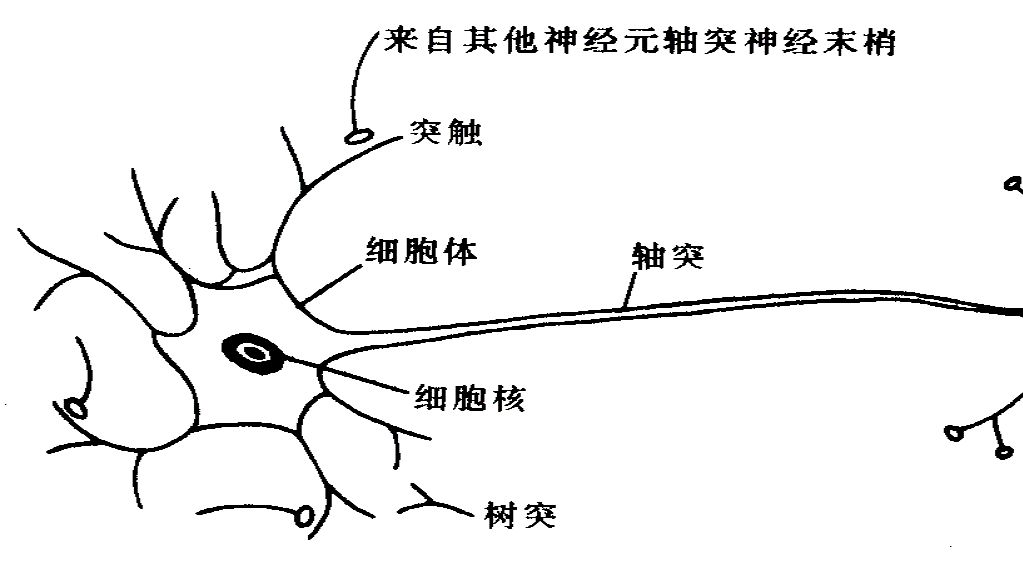
\includegraphics[width=14cm]{figure//1.png}
\caption{神经元信息的传递} \label{fig:1}
\end{figure}


\subsection*{大脑处理信息的特点}
\begin{itemize}
\item \textbf{分布存储与冗余性}: 记忆在大量元中,每个元存在许多信息的部分内容,信息在神经网络中的记忆反映在神经元间的突触连接强度上

\item \textbf{并行处理}: 经网络既是处理器又是存储器(并行处理不同于并行机)

\item \textbf{信息处理与存储合一}: 每个元兼有二者功能

\item \textbf{可塑性与自组织性}: 可塑性是学习记忆的基础

\item \textbf{鲁棒性}: 高连接度导致一定的误差和噪声不会使网络性能恶化。是智能演化的重要因素

\end{itemize}

\newpage
\section{人工神经网络(Artificial Neural Networks)
}
神经网络是一个并行和分布式的信息处理网络结构,它一般由许多个神经元组成,每个神经元只有一个输出,它可以连接到很多其他的神经元,每个神经元输入有多个连接通道,每个连接通道对应于一个连接权系数。

\begin{figure}[h]
\small
\centering
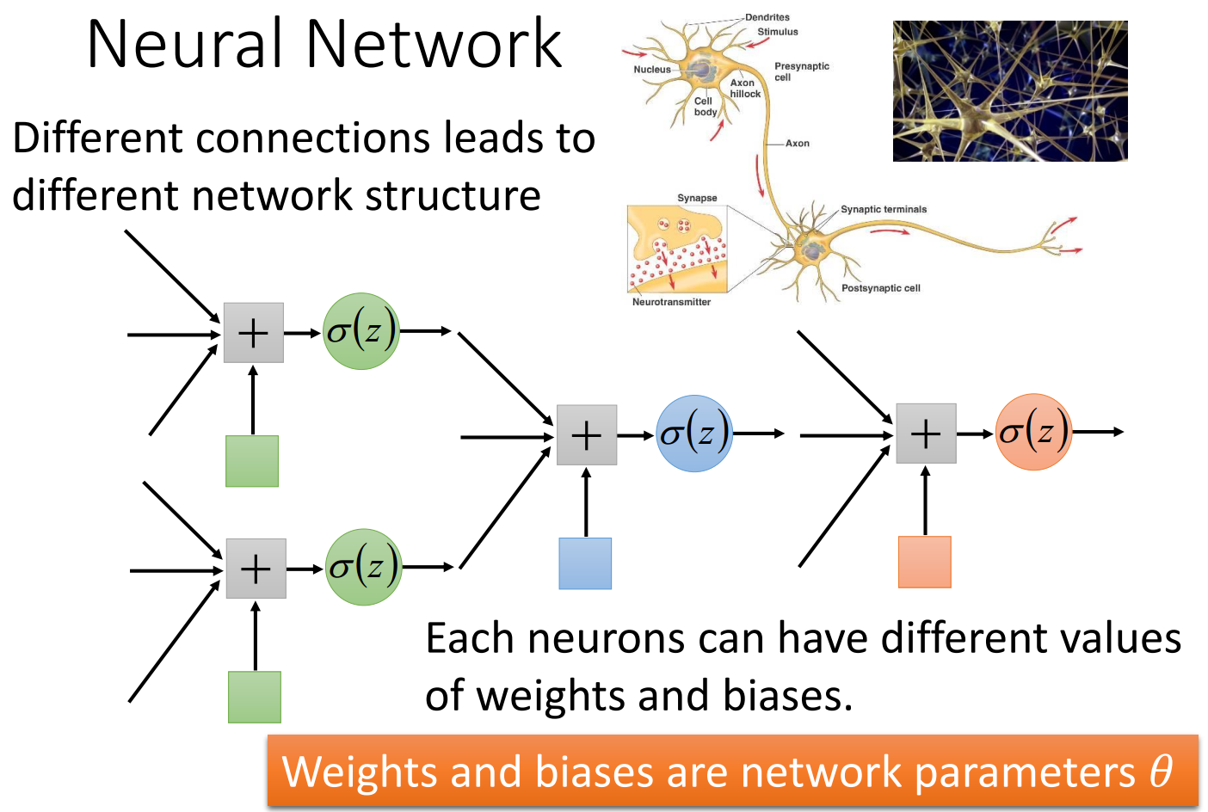
\includegraphics[width=16cm]{figure//2.png}
\caption{Artificial Neural Networks} \label{fig:2}
\end{figure}

\subsection{人工神经元模型}

神经网络中最基本的成分是\textcolor{blue}{神经元(neuron)模型},即上述定义中的“简单单元”。在生物神经网络中,每个神经元与其他神经元相连,当它“兴奋”时,就会向相连的神经元发送化学物质,从而改变这些神经元内的电位;如果某神经元的电位超过了一个\textcolor{blue}{"阈值”(threshold)},那么它就会被激活,即“兴奋"起来,向其他神经元发送化学物质。

1943年,[Mccu11ochandPitts,1943]将上述情形抽象为图所示的简单模型,这就是一直沿用至今的“M-P神经元模型”在这个模型中,神经元接收到来自n个其他神经元传递过来的输入信号,这些输入信号通过带权重的连接(connection)进行传递,神经元接收到的总输入值将与神经元的阈值进行比较然后通过\textcolor{blue}{“激活函数”(activation function)}处理已产生神经元的输出。

\begin{figure}[h]
\small
\centering
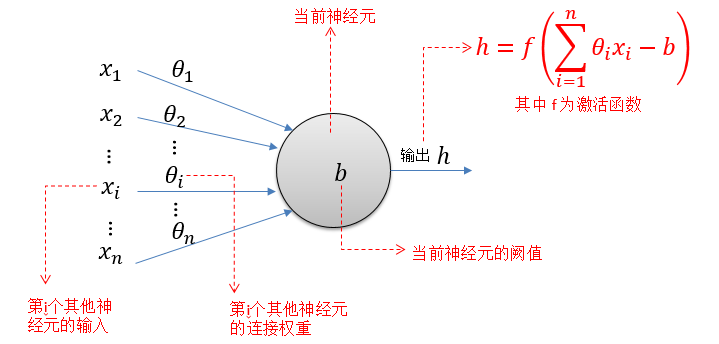
\includegraphics[width=14cm]{figure//3.png}
\caption{Artificial Neuron Model} \label{fig:3}
\end{figure}

\subsection*{激活函数}
理想中的激活函数$f(x)$是图(a)所示的阶跃函数,它将输入值映射为输出值“0”或“1”,“1”对应神经元兴奋,“0”对应神经元抑制。但是,阶跃函数具有不连续,不光滑(不连续可导)等不太好的性质\footnote{事实上在使用阶跃函数时,神经网络中的权值或偏置的微小改变可能会造成输出结果天翻地覆的变化,这使得网络的行为变得复杂且难以控制。},因此实际中常用Logistic回归中应用到的\textcolor{blue}{sigmoid函数}作为激活函数。典型的sigmoid函数如图(b)所示,它把可能在较大范围内变化的输入值挤压到(0,1)输出值范围内,因此有时又称之为“挤压函数”(squashing function).

\begin{figure}[h]
\small
\centering
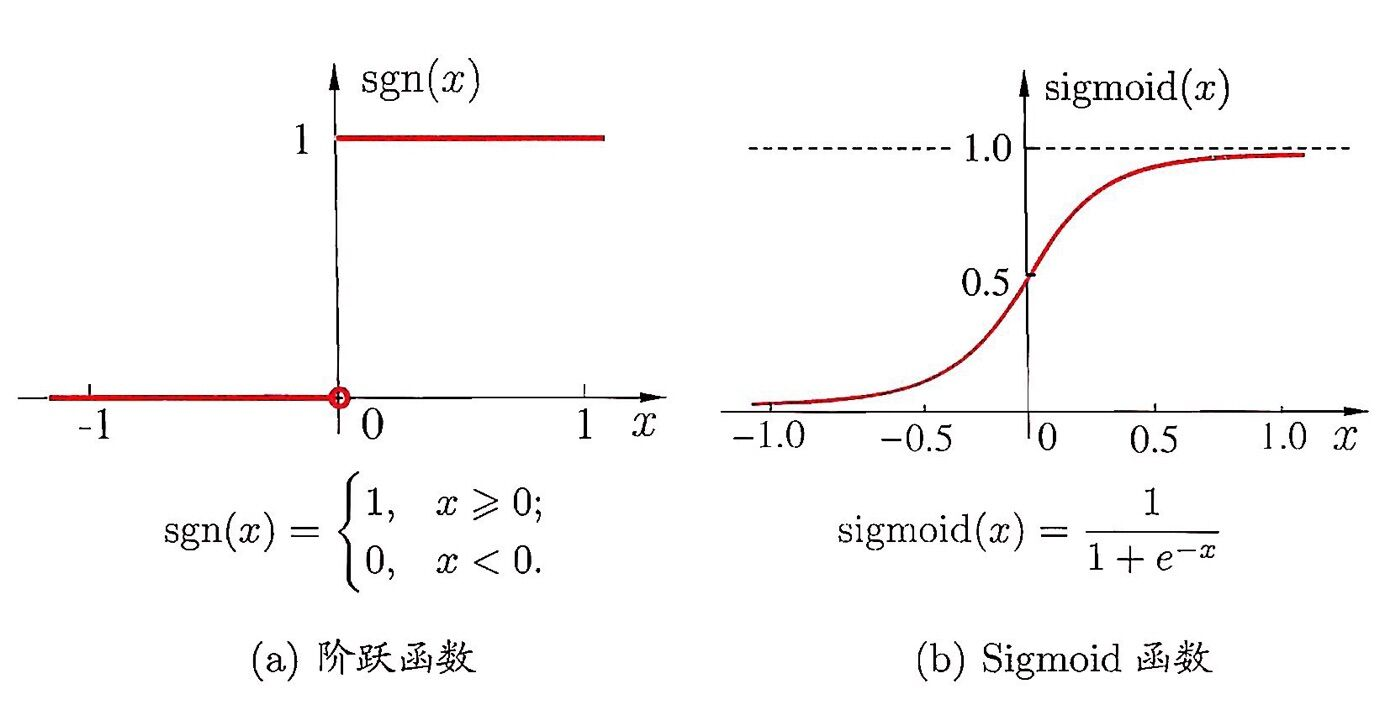
\includegraphics[width=14cm]{figure//4.jpg}
\caption{激活函数} \label{fig:4}
\end{figure}


\subsection{人工神经网络的构成}
\subsubsection{感知机(Perceptron)}

感知机(Perceptron)由两层神经元组成,如图所示,输入层接收外界输入信号后传递给输出层,输出层是M-P神经元,亦称"阈值逻辑单元"(threshold logic unit)

感知器处理单元对$n$个\textbf{二进制}输入$x_1,x_2,\ldots$,进行加权和操作并产生一个二进制输出:
\[\boxed{y=f\big(\sum_i w_ix_i-\theta\big)}\]

感知机能容易地实现逻辑\textbf{与、或、非}运算:

\begin{itemize}

\item 先定义$f(x)$为阶跃函数

\item “与”$(x_1\wedge x_2)$: 
令$w_1=w_2=1,\theta=2$;
则仅在$x_1=x_2=1$时,$y=1$;

\item “或”$(x_1\vee x_2)$: 
令$w_1=w_2=1,\theta=0.5$;
则仅在$x_1=x_2=1$时,$y=1$;

\item “非”$(\neg x_1)$: 
令$w_1=-0.6,w_2=0,\theta=-0.5$;
那么当$x_1=1$时,$y=0$;
\end{itemize}

\begin{figure}[h]
\small
\centering
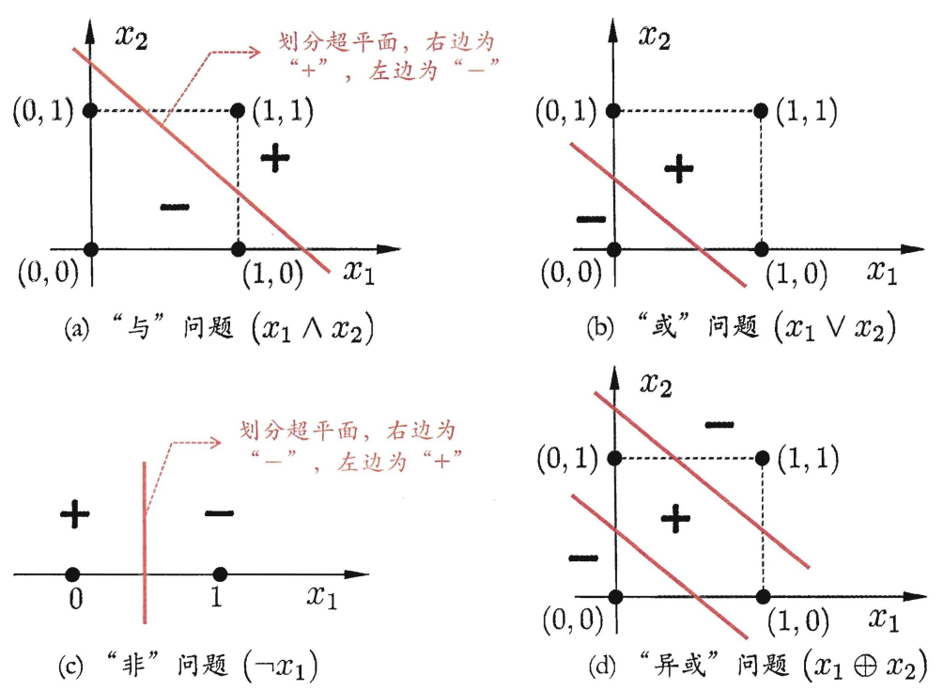
\includegraphics[width=14cm]{figure//5.png}
\caption{与、或、非运算的实现} \label{fig:5}
\end{figure}

需注意的是,感知机只有输出层神经元进行激活函数处理,即只拥有一层功能神经元 (functional neuron),其学习能力非常有限,只能处理\textcolor{red}{线性可分(linearly separable)}的问题。

从图中可以看出,与、或、非问题的分类样本是可以用一条直线分开的,即具有“线性可分”性质。

\subsubsection{多层感知机(MLP)}
\textcolor{red}{要解决非线性可分问题,就需考虑多层功能神经元。}

而“异或”问题的分类样本需要两条线才能将其分开,故需要两层感知机才能实现,如图1.6

\begin{figure}[h]
\small
\centering
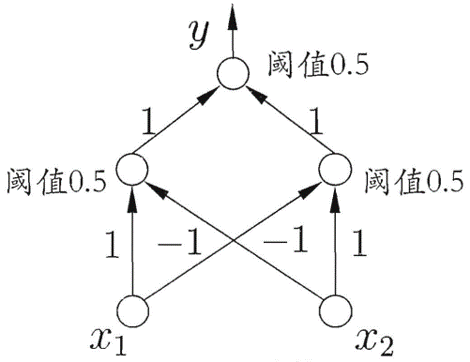
\includegraphics[width=6cm]{figure//6.png}
\caption{能解决异或问题的两层感知机} \label{fig:6}
\end{figure}

\begin{center}
  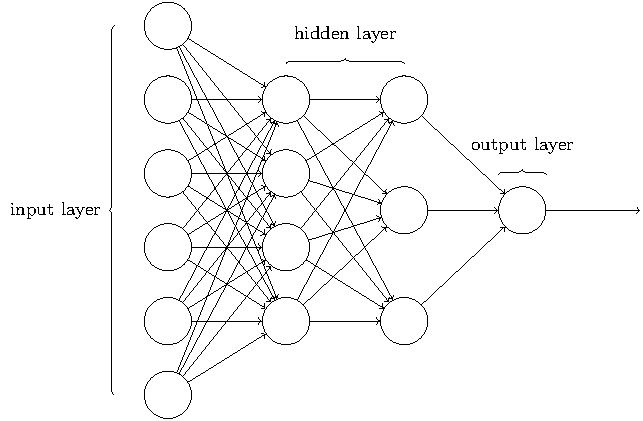
\includegraphics{figure//tikz11}
\end{center}

\begin{itemize}
\item 这个网络中最左边的称为\textbf{输入层},其中的神经元称为\textbf{输入神经元}。

\item 最右边的,即\textbf{输出层}包含有\textbf{输出神经元}。

\item 中间层,这层中的神经元既不是输入也不是输出,被称为\textbf{隐藏层}。 

\item 隐含层和输出层神经元都是拥有\textcolor{red}{激活函数}的功能神经元. 

\item 只需包含隐层,即可称为多层网络.神经网络的学习过程,就是根据训练数据来调整神经元之间的\textcolor{blue}{“连接权” (connection weight)}以及每个功能神经元的阈值;

\item 换言之,神经网络“学”到的东西,蕴涵在\textcolor{red}{连接权与阈值}中。

\end{itemize}
\subsection{人工神经网络的学习}

\begin{enumerate}
\item 试用数值方法求出$f(x, y)$在区域
$D = \{ (x,y)|0 \le x \le 0.8,0.5 \le y \le 1.5\}$上的一个近似表达式:

\[\boxed{p(x,y) = \sum\limits_{r,s = 0}^k {{c_{rs}}{x^r}{y^s}} }\]
要求$p(x,y)$最小的$k$值达到以下的精度:
\[\sigma  = \sum\limits_{i = 0}^{10} {\sum\limits_{j = 0}^{20} {(f({x_i},{y_j}) - p} } ({x_i},{y_j}){)^2} \le {10^{ - 7}}\]
其中,${x_i} = 0.08i,{y_j} = 0.5 + 0.05j$。

\item 计算$f(x_i^{\ast},y_j^{\ast}),p(x_i^{\ast},y_j^{\ast})\qquad (i = 1, 2,\cdots,8;j = 1,2,\cdots,5)$的值,以观察$p(x,y)$逼近$f(x,y)$的效果,其中,$x_i^{\ast}=0.1\bm{i},y_j^{\ast}=0.5+0.2\bm{j}$。
\end{enumerate}


\qd{说明}:
\begin{enumerate}
\item 用迭代方法求解非线性方程组时,要求近似解向量
${\bm{x}^{(k)}}$满足以下精度
\[\dfrac{\|{\bm{x}^{(k)}} - {\bm{x}^{(k - 1)}}\|_{\infty }}{\|{\bm{x}^{(k)}}\|_{\infty }} \le {10^{ - 12}}\]

\item 作二元插值时,要使用分片二次代数插值。

\item 要由程序自动确定最小的$k$值。

\item 打印以下内容:

\begin{enumerate}
\item 全部源程序;

\item 数表:$({x_i},{y_j},f({x_i},{y_j}))\qquad (i = 0,1,2,\cdots,10;j = 0,1,2,\cdots,20)$;

\item 选择过程的$k,\sigma$值;

\item 达到精度要求时的$k$和$\sigma$值以及$p(x,y)$中的系数
$c_{rs}(r = 0,1,\cdots,k;s = 0,1,\cdots,k)$;

\item 数表:$(x_i^{\ast},y_j^{\ast},f(x_i^{\ast},y_j^{\ast})),p(x_i^{\ast},y_j^{\ast})\qquad (i = 1, 2,\cdots,8;j = 1,2,\cdots,5)$。

\end{enumerate}
\item 采用$f$型输出$x_i,y_j,x_i^{\ast},y_j^{\ast}$的准确值,其余实型数采用$e$型输出并且至少显示12位有效数字。
\end{enumerate}


\newpage
\chapter{算法设计方案}
\section{方案}
\begin{enumerate}
\item 将${x_i} = 0.08i,{y_j} = 0.5 + 0.05j\quad (i=0,1,\cdots,10;j=0,1,\cdots,20)$代入方程组中,用Newton迭代法解出$t_{ij}$和$u_{ij}$;

\item 对数表$z(t,u)$进行分片二次代数插值,
求得$z_{ij}=f(t_{ij},u_{ij})$

\item 根据$z_{ij}$的值进行曲面拟合,得$p(x,y)$

\item 观察比较
\end{enumerate}
\newpage

\section{Newton迭代法}

\[\left\{ \begin{array}{l}
0.5\cos t + u + v + w - x = 2.67\\
t + 0.5\sin u + v + w - y = 1.07\\
0.5t + u + \cos v + w - x = 3.74\\
t + 0.5u + v + \sin w - y = 0.79
\end{array} \right.\]

对于该非线性方程组方程组来说,$x,y$为已知量,
需解出$t,u,v,w$。

设$\bm{x}= {(t,u,v,w)^T}$,并设定精度水平${\varepsilon } = {10^{ - 12}}$和最大迭代次数$M$

先在${\bm{x}^{\ast}}$附件选取${\bm{x}^{(0)}}= {({t^{(0)}},{u^{(0)}},{v^{(0)}},{w^{(0)}})^T}$

具体算法如下:
\begin{algorithm}[h]  
\caption{Newton's method}  
\begin{algorithmic}[1]  
\STATE Set $\bm{x}^{(0)}\in D$ and $k=0$
\WHILE {k<M}
\STATE Compute $\bm{F}(\bm{x}^{(k)})$ 
and $\bm{F}'(\bm{x}^{(k)})$
\STATE Compute $\Delta \bm{x}^{(k)}=-[\bm{F}'(\bm{x}^{(k))}]^{-1}\bm{F}(\bm{x}^{(k)})$
\IF {$\|\Delta \bm{x}^{(k)}\|/\|\bm{x}^{(k+1)}\|\le \varepsilon$}
\STATE $\bm{x}^{\ast}=\bm{x}^{(k)}$
\STATE Break
\ENDIF 
\STATE $\bm{x}^{(k+1)}= \bm{x}^{(k)}+
\Delta \bm{x}^{(k)}$
\STATE k=k+1
\ENDWHILE
\end{algorithmic}  
\end{algorithm}  




\section{分片双二次插值}




为了加快$QR$迭代的收敛速度, 我们可以采用位移策略和反迭代思想.
\begin{algorithm}[h]  
\caption{QR Iteration with shift}  
\begin{algorithmic}[1]  
\STATE Set $A_1=A$ and $k=1$
\WHILE {not convergence}
\STATE Choose a shift $\sigma_k$
\STATE ${A_{k}-\sigma_kI} = Q_k R_k$
\STATE Compute $A_{k+1}=R_k Q_k+\sigma_kI$
\STATE k=k+1
\ENDWHILE
\end{algorithmic}  
\end{algorithm}  

我们有
\begin{align*}
A_{k+1}=R_kQ_k+\sigma_kI&=(Q^T_kQ_k)R_kQ_k+\sigma_kI\\
&=Q^T_k(A_k-\sigma_kI)Q_k+\sigma_kI\\
&=Q^T_kA_kQ_k
\end{align*}

所以, 带位移的$QR$算法中所得到的所有矩阵$A_k$都与$A$正交相似.

\newpage
\chapter{问题求解}
\begin{enumerate}
\item 初始化定义$A$矩阵

\item 采用$Householder$变化将$A$矩阵拟上三角化得到矩阵$A^{n-1}$

\item 采用$QR$分解将矩阵$A^{n-1}$分解为矩阵Q与R,并打印RQ

\item 用带双步位移的QR方法求解所有特征值

\item 用Gauss消去法求解$(A-\lambda I)X=0$,得到对应的特征向量

\item 输出
\end{enumerate}
\newpage


\chapter{源程序}
\section{C语言版大作业}
\begin{lstlisting}[language=C]
#include<stdio.h>
#include<math.h>
#include<string.h>
#define N 20
const double eps=1e-12;
double a[N][N],B[N][N],C[N][N];
int n=10;

typedef struct{
//定义复数结构体
    double Re;
    double Im;
}ComplexNumber;

void zeroMat(double a[N][N]){
    for(int i= 1; i<=10; i++) {
        for(int j = 1; j<=10; j++) {
            if (fabs(a[i][j])<eps)
                a[i][j] = 0;
        }
    }
}

void def(){
	//初始化A数组
	for(int i=1;i<=n;i++)
		for(int j=1;j<=n;j++){
			if(i==j)
				a[i][j]=1.52*cos(i+1.2*j);
			else if(i!=j)
				a[i][j]=sin(0.5*i+0.2*j);
		}
}

void eye(double Q[N][N]){
	//定义单位阵 
	for(int i=1;i<=n;i++)
		for(int j=1;j<=n;j++)
			Q[i][j]=(i==j);
}

int Is_zero(double Q[N][N],int r,int k){
	//K>0表示在QR中调用,K<0表示在 DQR中调用 
	int kk=n;//更改数组大小 
	if(k<0){kk=-k;k=1;}
	for(int i=r+k;i<=kk;i++)
		if(fabs(Q[i][r])>eps)
			return 0;
	return 1;
}


int sgn(double x){
	if(x>0)
		return 1;
	return -1;
}

void Matirix_M(double A[N][N],double x[N],double y[N],double h){
	for(int i=1;i<=n;i++)y[i]=0;
	for(int i=1;i<=n;i++)
		for(int j=1;j<=n;j++)
			y[i]+=A[i][j]*x[j]/h;
}

double Vector_M(double x[N],double y[N]){
	double sum=0;
	for(int i=1;i<=n;i++)
		sum+=x[i]*y[i];
	return sum;
}

void MatirixM_M(double X[N][N],double Y[N][N]){
	for(int i=1;i<=n;i++)
		for(int j=1;j<=n;j++)
			for(int k=1;k<=n;k++)
				B[i][j]+=X[i][k]*Y[k][j];
}

void copy(double X[N][N],double Y[N][N]){
	for(int i=1;i<=n;i++)
		for(int j=1;j<=n;j++)
			X[i][j]=Y[i][j];
}

void output(double A[N][N]){
	for(int i=1;i<=n;i++){
		for(int j=1;j<=n;j++)
			printf("%.12e ",A[i][j]);
		printf("\n");
	}
}

void QR(double A[N][N],double Q[N][N]){
	double u[N],w[N],p[N],d,c,h;
	eye(Q);
	for(int r=1;r<n;r++){
		d=0;
		if(Is_zero(A,r,1))continue;
		for(int i=r;i<=n;i++)
			d+=A[i][r]*A[i][r];
		d=sqrt(d);
		c=-sgn(A[r][r])*d;
		h=c*c-c*A[r][r];
		for(int i=1;i<=n;i++){
			if(i<r)
				u[i]=0;
			else if(i==r)
				u[i]=A[r][r]-c;
			else if(i>r)
				u[i]=A[i][r];
		}
		memset(w,0,sizeof(w));
		Matirix_M(Q,u,w,1);
		for(int i=1;i<=n;i++)
			for(int j=1;j<=n;j++)
				Q[i][j]-=(w[i]*u[j]/h);
		memset(p,0,sizeof(p));
		for(int i=1;i<=n;i++)
			for(int j=1;j<=n;j++)
				p[i]+=(A[j][i]*u[j]/h);
		for(int i=1;i<=n;i++)
			for(int j=1;j<=n;j++)
				A[i][j]-=(u[i]*p[j]);
	}
}

void Householder_Triangularization(double A[N][N]){
	double u[N],p[N],q[N],d,c,h;
	for(int r=1;r<n-1;r++){
		d=0;
		if(Is_zero(A,r,2))continue;
		for(int i=r+1;i<=n;i++)
			d+=A[i][r]*A[i][r];
		d=sqrt(d);
		c=-sgn(A[r+1][r])*d;
		h=c*c-c*A[r+1][r];
		for(int i=1;i<=n;i++){
			if(i<=r)
				u[i]=0;
			else if(i==(r+1))
				u[i]=A[i][r]-c;
			else if(i>r)
				u[i]=A[i][r];
		}
		memset(p,0,sizeof(p));
		for(int i=1;i<=n;i++)
			for(int j=1;j<=n;j++)
				p[i]+=(A[j][i]*u[j]/h);
		Matirix_M(A,u,q,h);
		c=Vector_M(p,u)/h;
		for(int i=1;i<=n;i++)
			q[i]-=u[i]*c;
		for(int i=1;i<=n;i++)
			for(int j=1;j<=n;j++)
				A[i][j]-=(q[i]*u[j]+u[i]*p[j]);
	}
}


void select(int k,double b[N][N]){
	double max,c;
	int m=k;
	max=b[k][k];
	for(int i=k+1;i<=n;i++)
		if(fabs(b[i][k])>fabs(max)){
			max=b[i][k];
			m=i;
		}
	if(m!=k)
		for(int i=k;i<=n+1;i++){
		c=b[m][i];
		b[m][i]=b[k][i];
		b[k][i]=c;
		}
}

//Gauss消元法
void gauss(double lambda)
{
    double X[N];
    double m,sum,t;
    def();
    memset(X,0,sizeof(X));
    for(int i=1;i<=n;i++){
        a[i][i]-=lambda;
        a[i][n+1]=0;
    }
	for(int k=1;k<n;k++){
		select(k,a);
		for(int i=k+1;i<=n;i++){
			m=a[i][k]/a[k][k];
		for(int j=k;j<=n+1;j++)
			a[i][j]-=m*a[k][j];
		}	
	}
	X[n]=1;
	for(int i=n-1;i>=1;i--){
		sum=0;	
		for(int j=i+1;j<=n;j++) 
			sum+=a[i][j]*X[j];
		if(fabs(a[i][i])>eps)
			X[i]=(a[i][n+1]-sum)/a[i][i];
		else
			X[i]=0;
	}
	t=0;
	for(int i=1;i<=n;i++)
		t+=X[i]*X[i];
	t=sqrt(t);
	printf("Eigenvector=(");
	for(int i=1;i<=n;i++)
        printf("%lf ", X[i]/t);
    printf(")\n");
}

void DQR(double A[N][N]){
	double Q[N][N],M[N][N],s,t,re,im,a,b,c,d;
	double u[N],v[N],p[N],q[N],h,det;
	ComplexNumber L[N]; 
	int m=n,LL=1000,r=1;
	for(int k=1;k<=100;k++){
		if (m == 1) {
            L[r].Re = A[m][m];
            L[r].Im = 0; break;
        }
        else if(m<=0)break; 
		if(fabs(A[m][m-1])<=eps){
			L[r].Re = A[m][m];
            L[r].Im = 0;
            m--;r++;continue;
		}
		a=A[m-1][m-1];
		b=A[m-1][m];
		c=A[m][m-1];
		d=A[m][m];
		re=(a+d)/2;
		det=(a-d)*(a-d)+4*b*c;
		
		if((m==2)||(fabs(A[m-1][m-2])<=eps)){
			if(det>0){
				L[r].Re = re+sqrt(det)/2;
            	L[r].Im = 0;
            	L[r+1].Re = re-sqrt(det)/2;
            	L[r+1].Im = 0;
            }
            else if(det<0){
            	L[r].Re = re;
            	L[r].Im=sqrt(fabs(det))/2;
            	L[r+1].Re = re;
            	L[r+1].Im = -L[r].Im;
			}
            m-=2;
			r+=2;
			continue;
		}
		if(k==LL)break;
		s=a+d;
		t=a*d-c*b;
		memset(M,0,sizeof(M));
		for(int i=1;i<=m;i++)
			for(int j=1;j<=m;j++){
				for(int l=1;l<=m;l++)
					M[i][j]+=A[i][l]*A[l][j];
				M[i][j] -= s*A[i][j];
				M[i][j] += t*(i==j);
			}

		for(int r=1;r<m;r++){
			d=0;
			if(Is_zero(M,r,-m))continue;
			for(int i=r;i<=m;i++)
				d+=M[i][r]*M[i][r];
			d=sqrt(d);
			c=-sgn(M[r][r])*d;
			h=c*c-c*M[r][r];
			for(int i=1;i<=m;i++){
				if(i<r)
					u[i]=0;
				else if(i==r)
					u[i]=M[r][r]-c;
				else if(i>r)
					u[i]=M[i][r];
			}
			memset(p,0,sizeof(p));
			memset(q,0,sizeof(q));
			memset(v,0,sizeof(v));
			for(int i=1;i<=m;i++)
				for(int j=1;j<=m;j++)
					v[i]+=(M[j][i]*u[j]/h);	
			for(int i=1;i<=m;i++)
				for(int j=1;j<=m;j++){
					M[i][j]-=(u[i]*v[j]);
					p[i]+=(A[j][i]*u[j]/h);
					q[i]+=(A[i][j]*u[j]/h);
				}

			c=0;
			for(int i=1;i<=m;i++)
				c+=p[i]*u[i]/h;
			for(int i=1;i<=m;i++)
				q[i]-=u[i]*c;
			for(int i=1;i<=m;i++)
				for(int j=1;j<=m;j++)
					A[i][j]-=(q[i]*u[j]+u[i]*p[j]);
			zeroMat(A);
		}

	}
	zeroMat(A);
 	for(int r = 1; r<=10; r++){
        printf("\n");
        if (L[r].Im == 0) {
            printf("lambda[%d] = %.12e \n", r , L[r].Re); 
            gauss(L[r].Re);
        }
        else {
            printf("lambda[%d] = %.12e + i*%.12e\n", r , L[r].Re, L[r].Im);
        }
    }	
}

int main(){
	double Q[N][N];
	freopen("Works.in","r",stdin);
	freopen("Works.out","w",stdout);
	def();
	Householder_Triangularization(a);
	printf("A_n-1:\n");
	output(a);
	QR(a,Q);
	printf("\nR:\n");
	output(a);
	printf("\nQ:\n");
	output(Q);
	memset(B,0,sizeof(B));
	MatirixM_M(a,Q);
	printf("\nR*Q:\n");
	output(B);
	def();
	DQR(a);
	return 0;
}
\end{lstlisting}




\chapter{计算结果}
后面为输出结果:
\newpage


\newpage
特征值与向量如下:

$\lambda_{1}= 9.432879572769e-001$ 

Eigenvector=(0.079620,\quad 0.045421,\quad -0.018272,\quad -0.047961,\quad -0.349567,\quad 0.207215,\quad -0.152312,\quad 0.820634,\quad -0.355466,\quad 0.028866)


\vbox{}
$\lambda_{2}= 6.489488202110e-001$ 

Eigenvector=(0.108435,\quad 0.071344,\quad 0.382502,\quad -0.047100,\quad -0.717804,\quad 0.181519,\quad -0.226006,\quad 0.388381,\quad 0.289696,\quad 0.024333)


\vbox{}
$\lambda_{3}= -9.891143464725e-001$+ i*1.084758631513e-001


\vbox{}
$\lambda_{4}= -9.891143464725e-001$- i*1.084758631513e-001


\vbox{}
$\lambda_{5}= 4.954990923624e-002$ 

Eigenvector=(-0.213768,\quad -0.206774,\quad 0.386829,\quad -0.031112,\quad -0.380939,\quad -0.125174,\quad 0.644716,\quad -0.308201,\quad -0.295977,\quad 0.043723)


\vbox{}
$\lambda_{6}= -1.493147080915e+000$ 

Eigenvector=(-0.561341,\quad 0.778192,\quad 0.014364,\quad -0.277602,\quad 0.003568,\quad -0.002548,\quad -0.022061,\quad -0.011758,\quad -0.013173,\quad 0.035016)


\vbox{}
$\lambda_{7}= 1.590313458807e+000$ 

Eigenvector=(0.062377,\quad -0.011231,\quad -0.252846,\quad -0.130988,\quad -0.381985,\quad 0.815575,\quad -0.123377,\quad -0.067721,\quad 0.271945,\quad 0.100282)


\vbox{}
$\lambda_{8}= -2.336865932238e+000$+ i*8.934379210213e-001


\vbox{}
$\lambda_{9}= -2.336865932238e+000$- i*8.934379210213e-001


\vbox{}
$\lambda_{10}= 3.389613438816e+000$ 

Eigenvector=(-0.104872,\quad -0.217677,\quad -0.474694,\quad -0.259384,\quad -0.304665,\quad -0.259452,\quad 0.086866,\quad 0.405258,\quad 0.509628,\quad 0.239515)

\chapter{讨论}
\normalsize
1.在对$n\times n$实矩阵$\bm{A}$作QR分解或双步位移分解时不需要形成具体的矩阵$\bm{H}_i$,这样可以避免矩阵与矩阵相乘,大大减少了计算量。

2.在QR分解中,R矩阵可以直接储存在A的上三角部分,而在$M_k$的QR分解中,不需要再生成$\bm{B},\bm{C}$矩阵,直接在$\bm{M},\bm{A}$矩阵中迭代即可,以节约储存空间。

3.QR方法适用于计算一般实矩阵的全部特征值,但对于大型实矩阵,则收敛速度不够用了,这时我们为了加速收敛,可以引入位移量,通常, 位移越离特征值越近,收敛速度就越快,如果位移$\sigma$与某个特征值非常接近, 则$\bm{A}_{n,n}^{(k)}-\sigma$就非常接近于0.
这说明$\bm{A}_{n,n}^{(k)}$通常会首先收敛到$\bm{A}$的一个特征值.所以令$\sigma=\bm{A}_{n,n}^{(k)}$是一个不错的选择.
但是, 如果这个特征值是复数, 这种位移选取方法就可能失效.

假设$\sigma \in \mathbb{C}$是 $\bm{A}$ 的某个复特征值 $\lambda$ 的一个很好的近似, 则其共轭$\overline{\sigma}$也应
该是$\overline{\lambda}$的一个很好的近似. 因此我们可以考虑\qd{双位移策略}, 即先以$\sigma$为位移迭代一次, 然后再以$\overline{\sigma}$ 为位移迭代一次, 如此不断交替进行迭代.
这样就有
\begin{align*}
A_1-\sigma I&=Q_1R_1, \\
A_2&=R_1Q_1+\sigma I,\\
A_2-\overline{\sigma}I&=Q_2R_2, \\
A_3&=R_2Q_2+\overline{\sigma}I.
\end{align*}
容易验证
\[A_3=Q_2^TA_2Q_2=Q_2^{\ast}Q_1^{\ast}A_1Q_1Q_2=Q^{\ast}A_1Q,
\]
其中$Q=Q_1Q_2$.

我们注意到$\sigma$可能是复的, 所以 $Q_1$ 和 $Q_2$ 都可能是复矩阵. 但我们却可以
选取适当的 $Q_1$ 和 $Q_2$, 使的 $Q=Q_1Q_2$ 是实正交矩阵
从而$A_3 = Q^T A_1Q $也是实矩阵. 因此我们无需计算 $A_2$, 而是直接由 $A_1$ 计算出$A_3$.

4.最后,在用Gauss消去法求解$(A-\lambda I)X=0$,求得到对应的特征向量
时,需要将$X[n]$预设为1,因为由于线性方程组$AX=b$中的$b$向量全为0,所以解的自由度为1,需要自己先将$X[n]$的值定下来,才能迭代出剩下的解,不然求出的的解全为0.

\end{document}